\chapter{Kelengkapan Internship dan Tugas Akhir}

\section{Tahapan Pergantian Judul}
Lhat pada gambar \ref{figure:P2}.
\begin{figure}[ht]
	\centerline{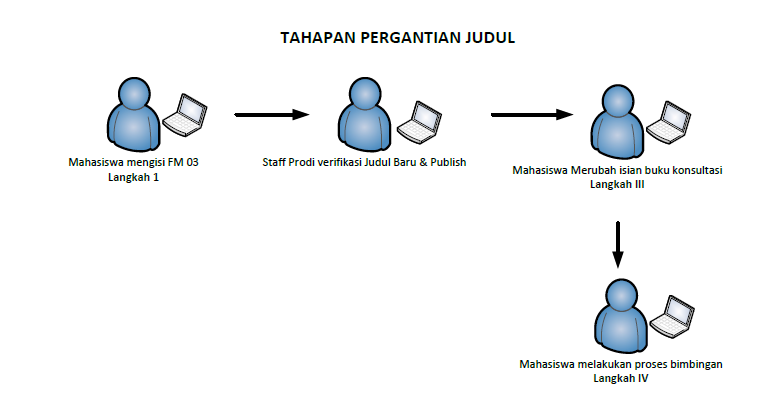
\includegraphics[width=1\textwidth]{figures/ganti_judul.png}}
	\caption{Tahapan Pergantian Judul}
	\label{figure:P2}
	\end{figure}

\section{Tahapan Pengajuan Sidang}
Lhat pada gambar \ref{figure:P3}.
\begin{figure}[ht]
	\centerline{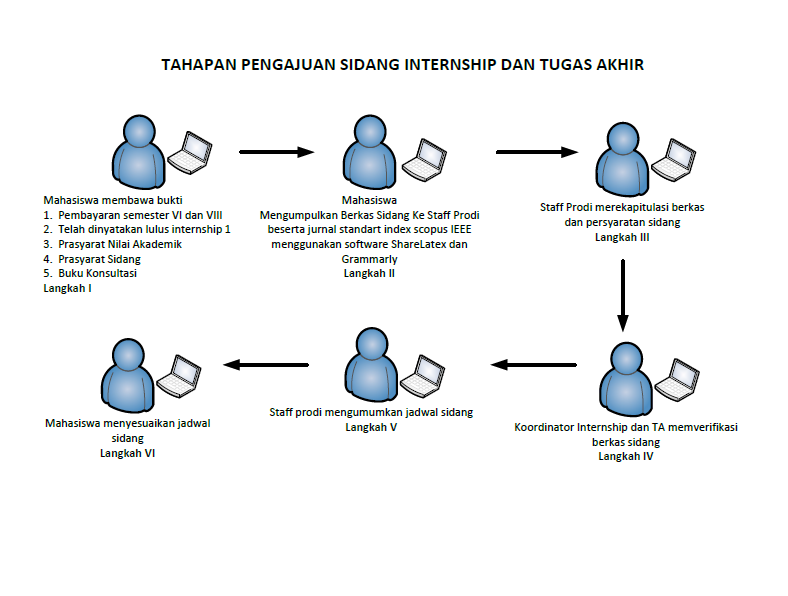
\includegraphics[width=1\textwidth]{figures/draft.png}}
	\caption{Tahapan Pengajuan Sidang}
	\label{figure:P3}
	\end{figure}
\section{Tahapan Revisi Laporan dan Jurnal}
Lhat pada gambar \ref{figure:P31}.
\begin{figure}[ht]
	\centerline{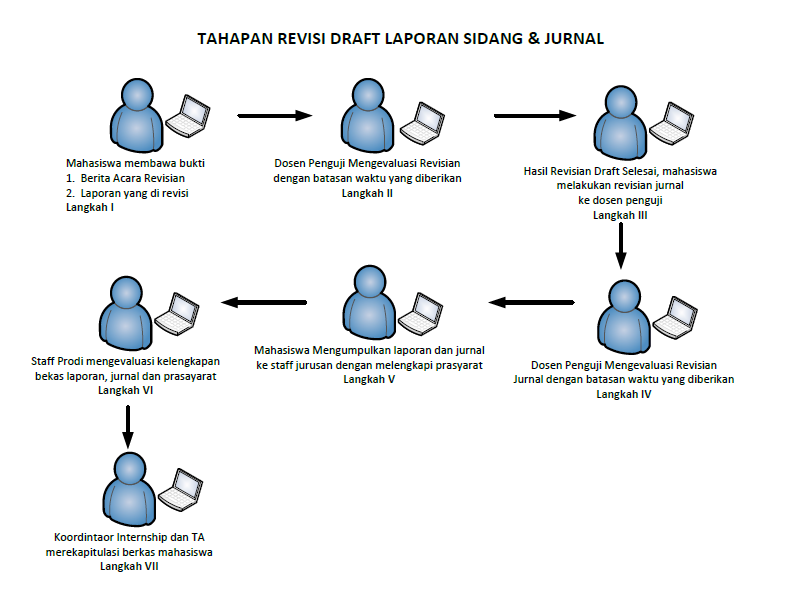
\includegraphics[width=1\textwidth]{figures/revisi.png}}
	\caption{Tahapan Revisi Laporan dan Jurnal}
	\label{figure:P31}
	\end{figure}
\section{Tahapan Sidang Ulang}
Lhat pada gambar \ref{figure:P4}.
\begin{figure}[ht]
	\centerline{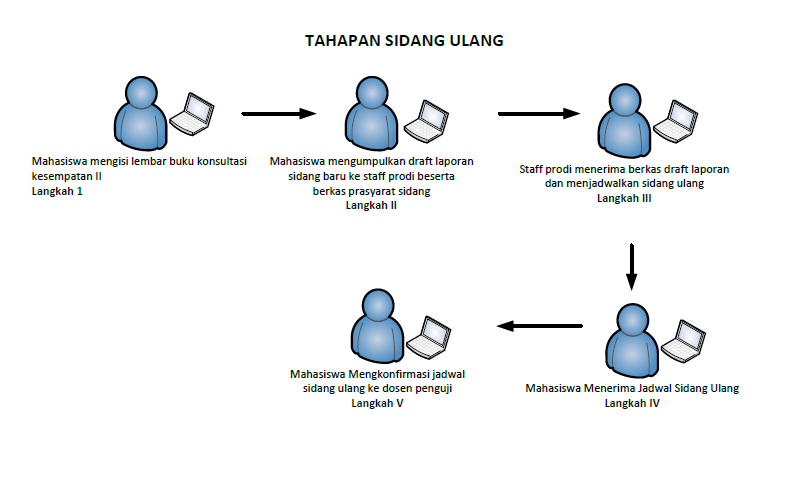
\includegraphics[width=1\textwidth]{figures/ulang.png}}
	\caption{Tahapan Sidang Ulang}
	\label{figure:P4}
	\end{figure}
\section{Tahapan Sidang Kode Etik}
Lhat pada gambar \ref{figure:P5}.
\begin{figure}[ht]
	\centerline{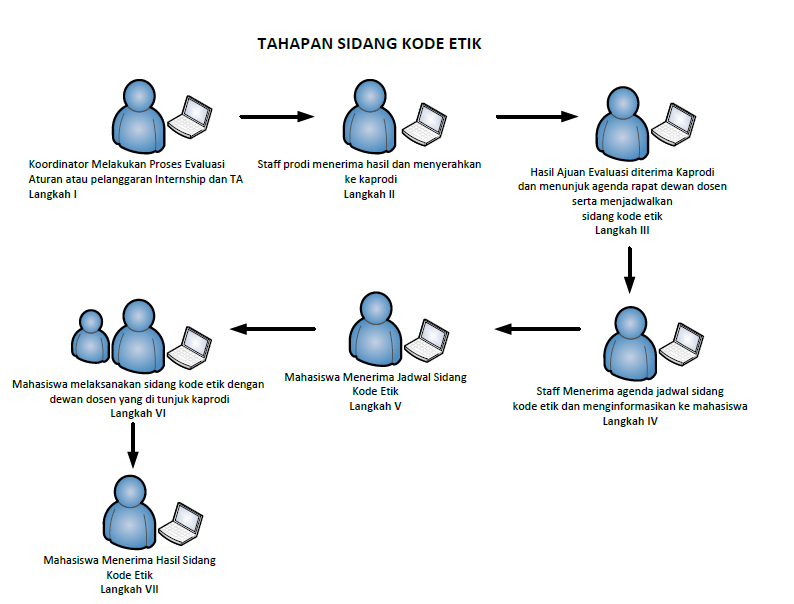
\includegraphics[width=1\textwidth]{figures/kode.png}}
	\caption{Tahapan Sidang Kode Etik}
	\label{figure:P5}
	\end{figure}
	
	
\chapter{Pengajuan Sidang dan Publikasi}

\section{Sidang dan Publikasi Tugas Akhir}
Pra-syarat penyelenggaran sidang dan publikasi antara lain:
\begin{enumerate}
	\item melengkapi data dan mencetak form sidang yang ada di menu Intranet portal if. Untuk yang metode publikasi, tanggal sidang diganti dengan tanggal diterimanya artikel pada jurnal tujuan. 
	\item Form sidang dimasukkan ke dalam Map Plastik Warna merah(lihat gambar \ref{mapplastik}), pada plastik bagian luar, depan di pojok kanan atas ditempel stiker label (lihat gambar \ref{label}) yang berisi nomor urut dari form penilaian tingkat akhir tab Tugas Akhir, Nama, NPM, Pembimbing I dan II yang diketik dan di print rapih pada stiker(lihat gambar \ref{labelcon}). Lampirkan juga surat diterimanya jurnal untuk diterbitkan(Jika ada).
	\item Pastikan oleh anda sendiri pembimbing sudah mengisi jadwal sidang di kolom Nilai Tingkat Akhir tab Tugas Akhir.
\end{enumerate}

\begin{figure}[ht]
	\centerline{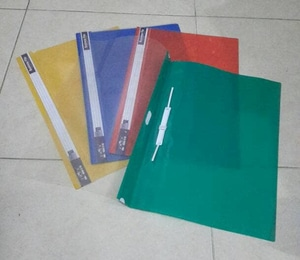
\includegraphics[width=.25\textwidth]{figures/mapplastik}}
	\caption{Map Plastik}
	\label{mapplastik}
	\end{figure}
	
	\begin{figure}[ht]
		\centerline{
\includegraphics[width=.25\textwidth]{figures/label}}
		\caption{Stiker Label}
		\label{label}
		\end{figure}

		\begin{figure}[ht]
			\centerline{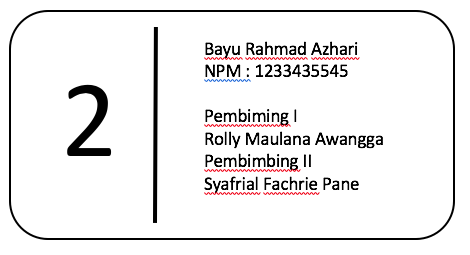
\includegraphics[width=.25\textwidth]{figures/labelcon}}
			\caption{Contoh Penulisan di Stiker}
			\label{labelcon}
			\end{figure}


Metode penilaian tugas akhir mahasiswa berhak untuk memilih dua metode, yaitu metode sidang dan publikasi.
\subsection{Metode Sidang}
Metode pertama adalah metode sidang. Metode sidang hanya diperbolehkan untuk mahasiswa dengan nilai akhir C. 
Pengajuan Jadwal Sidang TA silahkan berkordinasi dengan kedua pembimbing dan input langsung oleh pembimbingnya hari tanggal dan jamnya pada form nilai tingkat akhir tab Tugas AKhir. Pada saat sidang pastikan membawa map plastik yang sudah lengkap formnya. Membawa laporan, jurnal, dan slide PPT. Beberapa ketentuan standar pelaksanaan sidang yang wajib dipenuhi antara lain: 
\begin{enumerate}
	\item Form Pada Map sudah dilengkapi
	\item pada slide presentasi; Font ukuran minimal 24. Tidak boleh kurang dari ukuran font 24.
	\item pada slide presentasi; Paparkan referensi terlebih dahulu, kenapa memilih alasan referensi tersebut di daftar pustaka. Kemudian sebutkan target publikasi jurnalnya.
	\item Perlihatkan hasil scan plagiarisme dari laporan dan jurnal.
	\item Bawakan dan Sampaikan dalam bahasa Inggris selama sidang.
	\item Sampaikan presentasi dengan waktu kurang dari 10 menit. Pastikan anda membawa stop watch atau HP yang memiliki timer dengan settingan 10 menit.
\end{enumerate}
Selesai sidang, jika terdapat revisi maka selesaikan sebelum jangka waktu yang ditentukan. Untuk publikasi status sudah diterima maksimal sebelum jadwal UAS.

\subsection{Metode Publikasi}
Metode kelulusan dengan publikasi merupakan salah satu metode yang digunakan oleh perguruan tinggi di Australia dalam meluluskan mahasiswanya.
Dengan metode ini mahasiswa tidak diperlukan untuk melakukan sidang. Mahasiswa cukup mempublikasikan hasil karya ilmiahnya ke dalam ketiga kategori penilaian :
\begin{enumerate}
	\item Nilai A : Untuk kesanggunapan publikasi pada jurnal Internasional bereputasi.
	\item Nilai B : Untuk jurnal nasional Terakreditasi.
	\item Nilai C : Untuk Jurnal nasional terindeks DOAJ
\end{enumerate}

\subsection{Pernyataan Kelulusan}
Anda sudah dinyatakan lulus tanpa syarat jika Kolom Status Publikasi pada Nilai Tingkat Akhir tab Tugas Akhir sudah diubah oleh pembimbing menjadi SUDAH. Jika anda masih memiliki status publikasi BELUM, maka anda tidak berhak mengikuti wisuda dan mengambil ijasah atau surat keterangan lulus. Sehingga anda juga belum diperkenankan menggunakan gelar S.Tr.Kom. Apabila kami mendapati anda menggunakan gelar tanpa pernyataan kelulusan dari pembimbing, maka akan kami sediakan form pengunduran diri.


\chapter{Penutup}

Setiap mahasiswa  diwajibkan mengikuti ketentuan yang ditetapkan dalam buku pedoman ini. Dengan demikian diharapkan akan tercipta keseragaman format dan mutu laporan internship dan tugas akhir di lingkungan Program Studi D4 Teknik Informatika. Sejalan dengan perkembangan ilmu pengetahuan, Pedoman ini akan senantiasa disempurnakan. Oleh sebab itu, saran perbaikan akan dengan senang hati ditampung demi penyempurnaan buku pedoman ini. Hal yang belum diatur dalam pedoman ini akan ditetapkan kemudian.